
\sektion{Introduction to Gadsu}

%%%%%%%%%%%%%%%%%%%%%%%%%%%%%%%%%%%%%%%%%%%%%%%%
\fullimageCapt{gadse}{This is a cat.}{8cm}

%%%%%%%%%%%%%%%%%%%%%%%%%%%%%%%%%%%%%%%%%%%%%%%%
\fullimageCapt{shiatsu1white}{This is Shiatsu \ldots}{5.0cm}

%%%%%%%%%%%%%%%%%%%%%%%%%%%%%%%%%%%%%%%%%%%%%%%%
\fullimageCapt{shiatsu2ohashi}{\ldots so is this.}{6.3cm}

%%%%%%%%%%%%%%%%%%%%%%%%%%%%%%%%%%%%%%%%%%%%%%%%
\frame{\frametitle{Gadsu is \ldots} 
\pause
\begin{center}
\begin{Huge}
\textbf{Gad}se
\pause

\vspace{0.5cm}

+ Shiat\textbf{su}
\pause

\vspace{0.8cm}

= \textbf{Gadsu}
\end{Huge}
\end{center}

}

%%%%%%%%%%%%%%%%%%%%%%%%%%%%%%%%%%%%%%%%%%%%%%%%
\frame{\frametitle{Shiatsu is \ldots}

\begin{itemize}
	\item Acupressure
	\item Meridian therapy
	\item Physio therapy
	\item Massage
	\item Nervous System stimulation
	\item Based on the \textbf{T}raditional \textbf{C}hinese \textbf{M}edicine
	\begin{itemize}
		\item Concept of \textbf{Qi} flowing through the body and everything
		\item Every aspect of the human grouped into \textbf{5 Elements}
		\item Body and mind seen as a unit, not separated from each other
	\end{itemize}
\end{itemize}

\begin{figure}[h]
\centering
  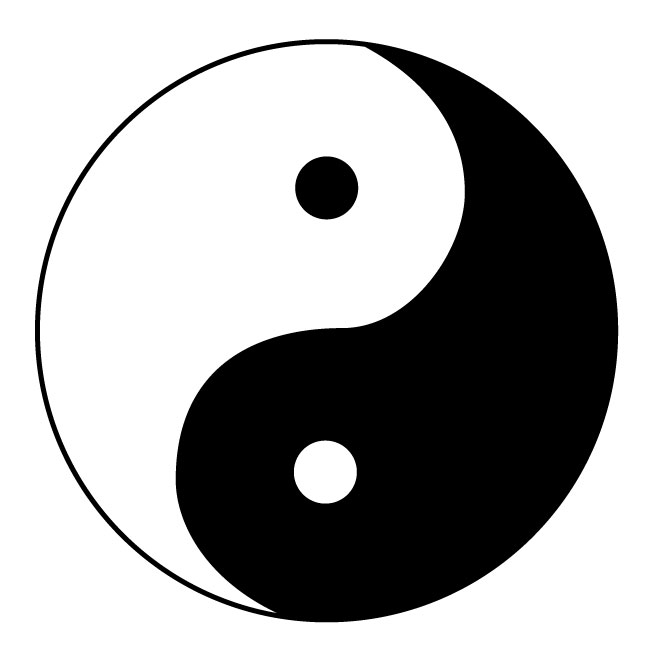
\includegraphics[height=2.0cm]{yinyang}
  \caption{Taiji Symbol, Theory of Yin Yang}
\end{figure}
}

%%%%%%%%%%%%%%%%%%%%%%%%%%%%%%%%%%%%%%%%%%%%%%%%
\begin{frame}[t]
\frametitle{Gadsu can \ldots}
\begin{columns}[t]
\begin{column}{0.5\textwidth}
	\textbf{Features:}
	\begin{itemize}
		\item Client database
		\item Manage medical records
		\item Generate reports
		\item Google integration
		\item Auto update, auto backup
	\end{itemize}
\end{column}
\begin{column}{0.5\textwidth} 
	\textbf{Roadmap:}
	\begin{itemize}
		\item Pain indicator, 5 Elements
		\item TCM software agent
		\item Statistics
		\item Invoicing
		\item Doodle integration
	\end{itemize}
\end{column}
\end{columns}
\end{frame}

%%%%%%%%%%%%%%%%%%%%%%%%%%%%%%%%%%%%%%%%%%%%%%%%
\begin{frame}
\frametitle{Technology Stack}
\begin{itemize}
	\item Gradle
	\item Swing
	\item Guice
	\item Spring JDBC
	\item HSQLDB + Flyway
	\item Jasper, Pdfbox
	\item Freemarker
	\item TestNG, Mockito, Hamcrest
	\item UISpec4J
	\item \textit{Initial implementation used Kotlin 0.6 $;)$}
\end{itemize}
\end{frame}


%%%%%%%%%%%%%%%%%%%%%%%%%%%%%%%%%%%%%%%%%%%%%%%%
\fullimageCapt{gadsu_screenshot}{\footnotesize{\textit{Gadsu got something like 35,000 LoC.}}}{11cm}


%%%%%%%%%%%%%%%%%%%%%%%%%%%%%%%%%%%%%%%%%%%%%%%%
\fulltitle{Let's have a look \ldots}
%\begin{whiteframe}
%haha
%\end{whiteframe}

